\appendixChapterTitle{ค}{การใช้งาน Vercel Cloud Deploy}
\vspace*{-0.8in}

\section{การใช้งาน Vercel}
\hspace*{1.3em}
Vercel คือแพลตฟอร์ม Cloud สำหรับนักพัฒนาเว็บที่เน้นความเร็วและความง่ายในการ Deploy\vspace{0.5em}

\begin{mycustomenum2}

\begin{figure}[H]
\centering
\adjustbox{frame, width=1.0\textwidth}{
    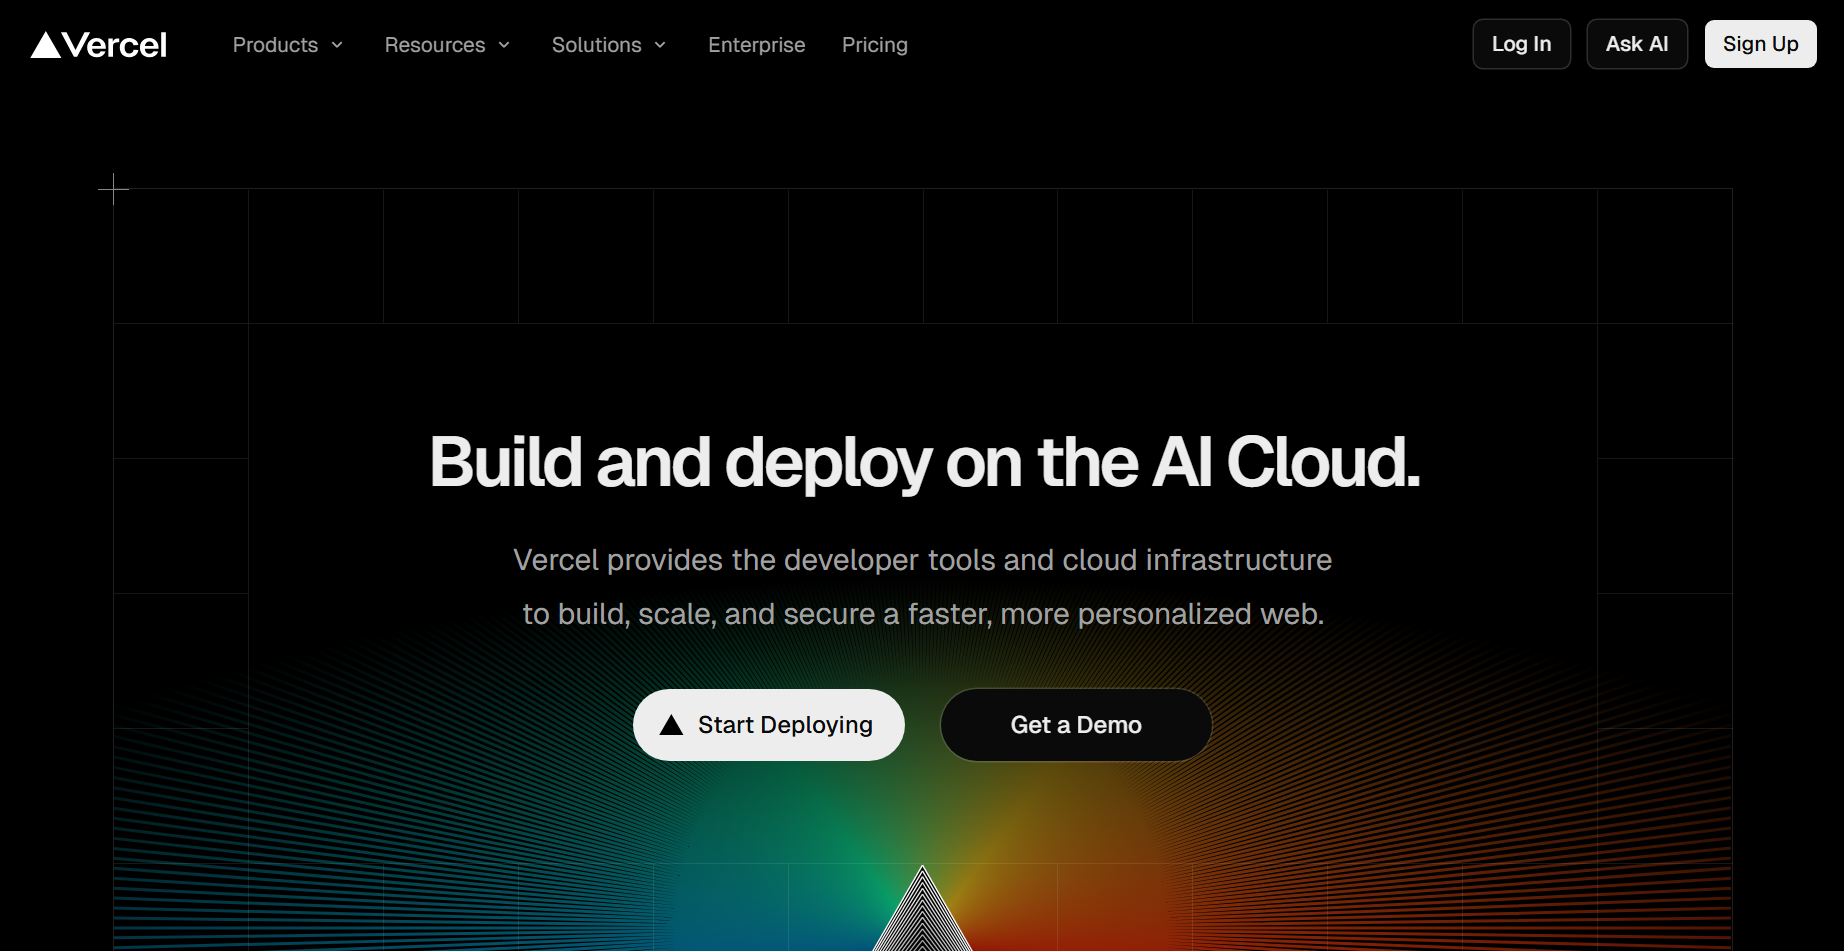
\includegraphics[width=1.0\textwidth]{Image/vercel.png}
}
\caption{\fontSixTeen{หน้าแรกของเว็บไซต์ Vercel}}
\item ไปที่เว็บไซต์ Vercel (\href{https://vercel.com/}{https://vercel.com/}) ตัวอย่างหน้าเว็บไซต์ Vercel
\item จากภาพที่ \ref{figB:Vercel1} ให้คลิกที่ \enquote{Sign Up} มุมขวาบนก็จะพบกับหน้าจอดังภาพที่ \ref{figB:vercel2}
\label{figB:Vercel1}
\end{figure}

\begin{figure}[H]
\centering
\adjustbox{frame, width=1.0\textwidth}{
    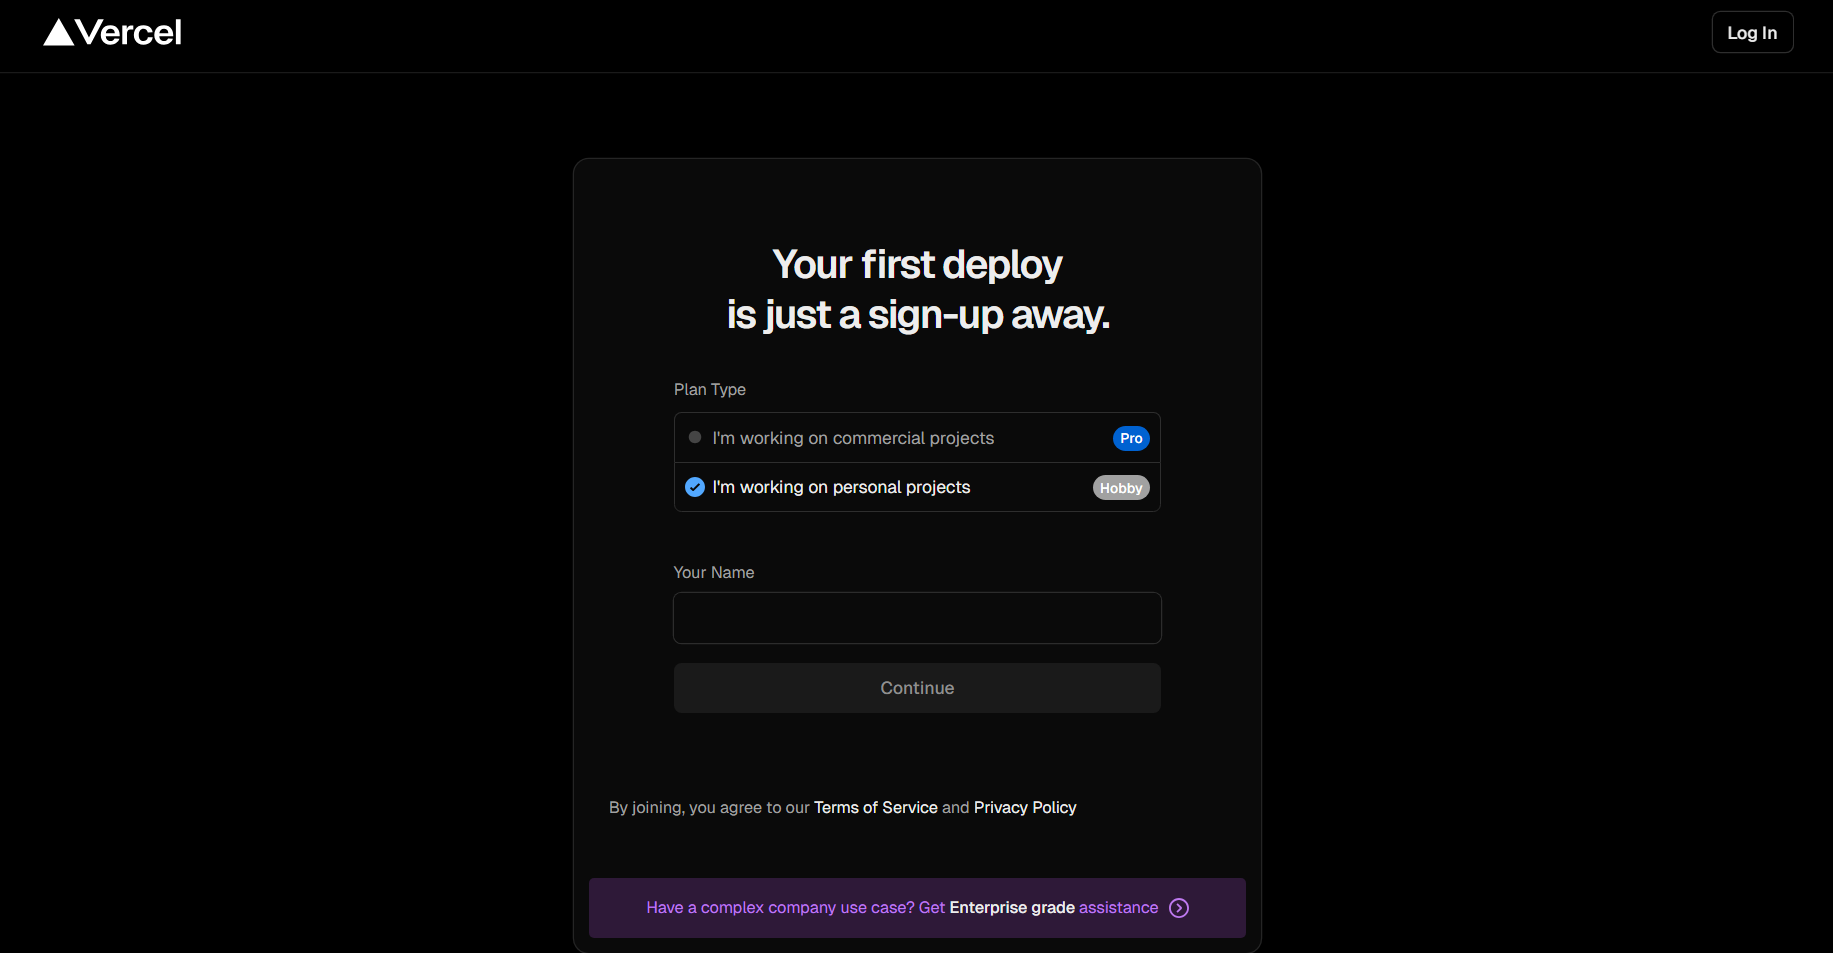
\includegraphics[width=1.0\textwidth]{Image/vercel-signup1.png}
}
\caption{\fontSixTeen{หน้า Sign Up ของเว็บไซต์ Vercel}}
\label{figB:Vercel2}
\end{figure}

\begin{figure}[H]
\centering
\adjustbox{frame, width=1.0\textwidth}{
    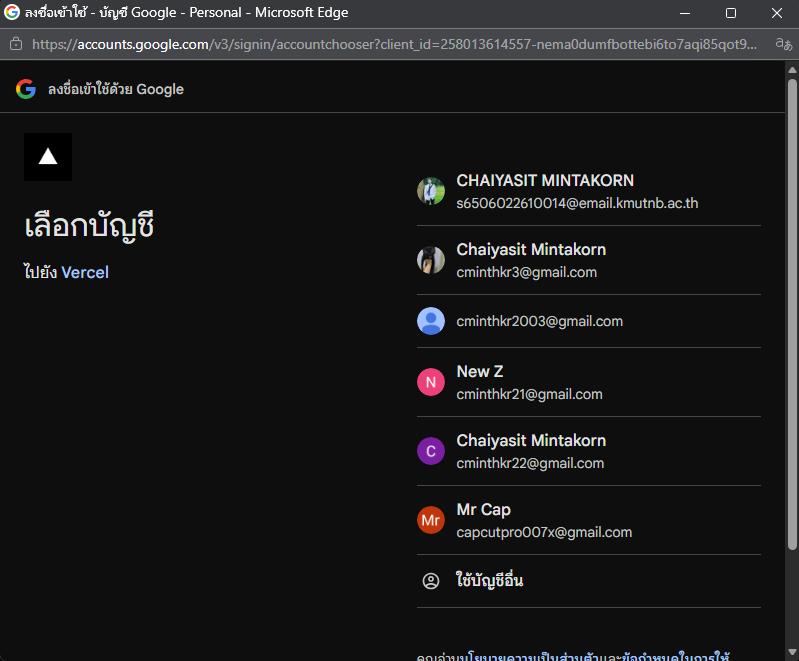
\includegraphics[width=1.0\textwidth]{Image/vercel-signup2.png}
}
\caption{\fontSixTeen{หน้าเลือกบัญชี Google สำหรับสมัครสมาชิกด้วย Google mail}}
\label{figB:Vercel3}
\end{figure}

\begin{figure}[H]
\centering
\adjustbox{frame, width=1.0\textwidth}{
    
\includegraphics[width=1.0\textwidth]{Image/vercel-signup3.png}
}
\caption{\fontSixTeen{หน้ายืนยันให้ Vercel เข้าถึงข้อมูล}}
\label{figB:Vercel4}
\end{figure}

\begin{figure}[H]
\centering
\adjustbox{frame, width=1.0\textwidth}{
    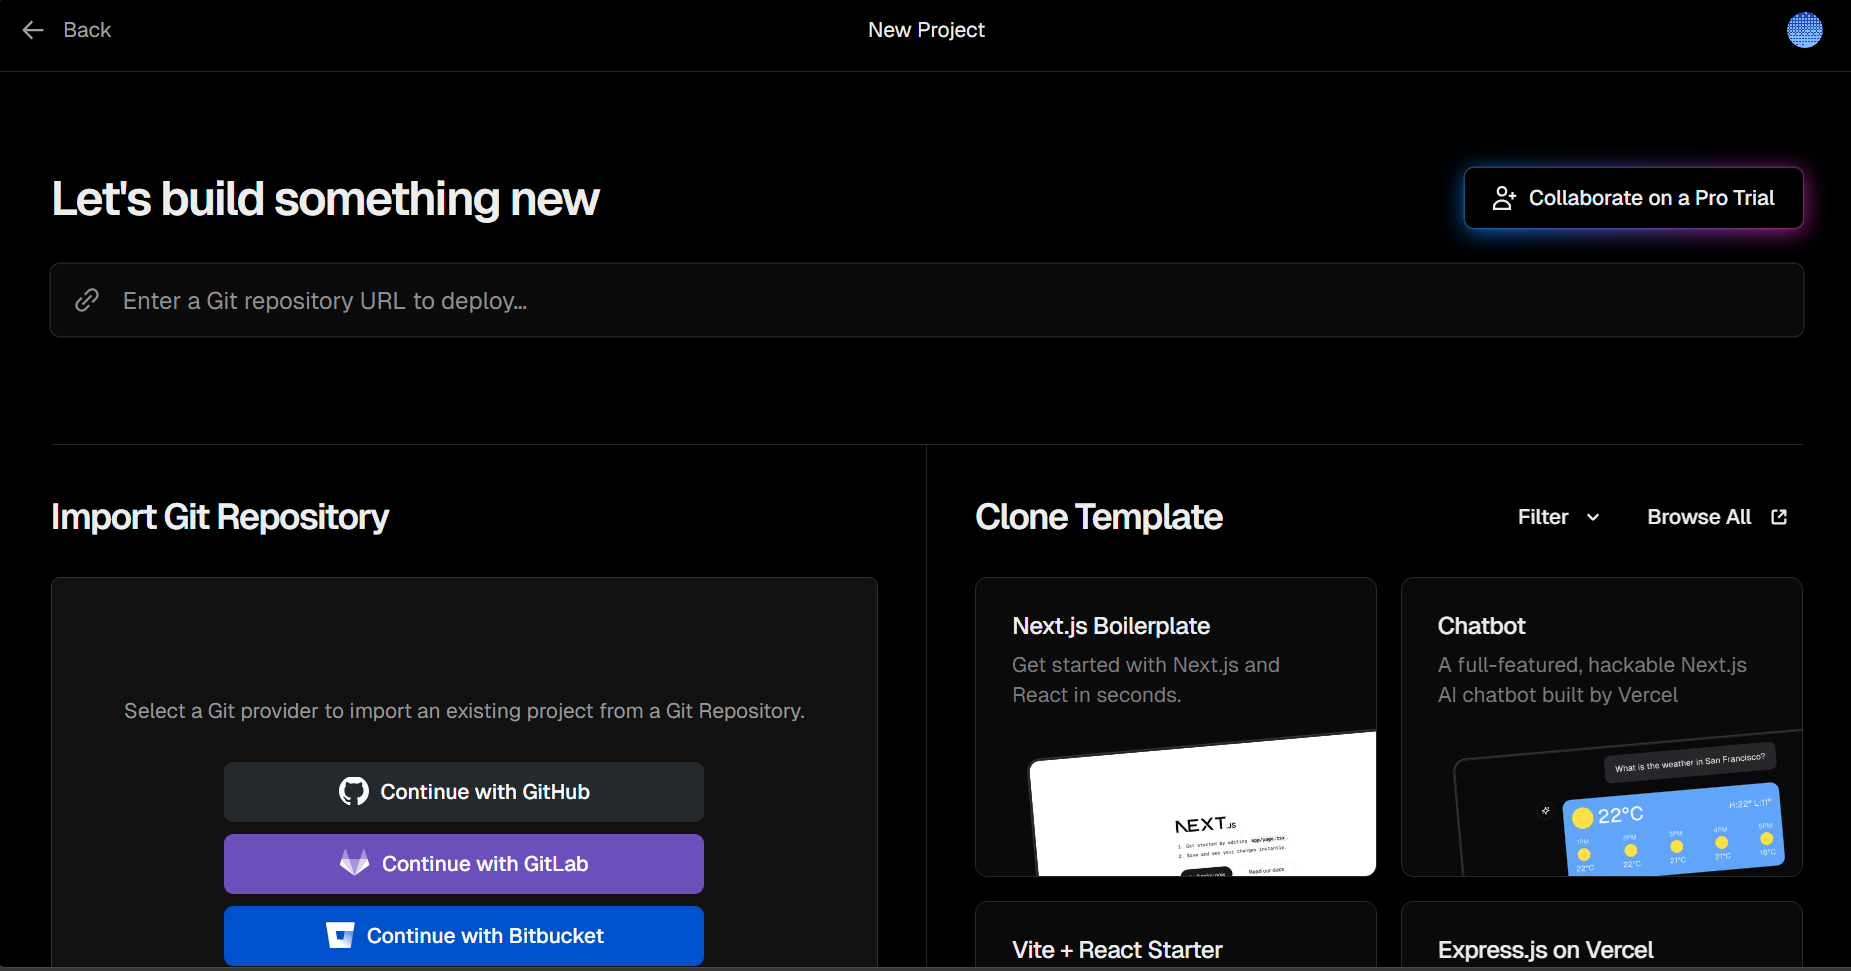
\includegraphics[width=1.0\textwidth]{Image/vercel-1.png}
}
\caption{\fontSixTeen{หน้าหลังจากสมัครบัญชีเสร็จ}}
\label{figB:Vercel5}
\end{figure}
\item จากภาพที่ \ref{figB:Vercel5} ให้คลิกที่ \enquote{Continue with GitHub} เพื่อเชื่อมต่อบัญชี GitHub สำหรับ Import Repository

\begin{figure}[H]
\centering
\adjustbox{frame, width=1.0\textwidth}{
    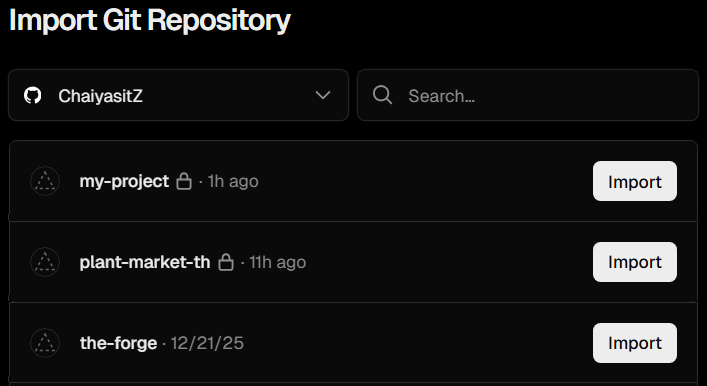
\includegraphics[width=1.0\textwidth]{Image/vercel-2.png}
}
\caption{\fontSixTeen{เลือก Import สำหรับ Repository ที่ต้องการ}}
\label{figB:Vercel6}
\end{figure}

\begin{figure}[H]
\centering
\adjustbox{frame, width=1.0\textwidth}{
    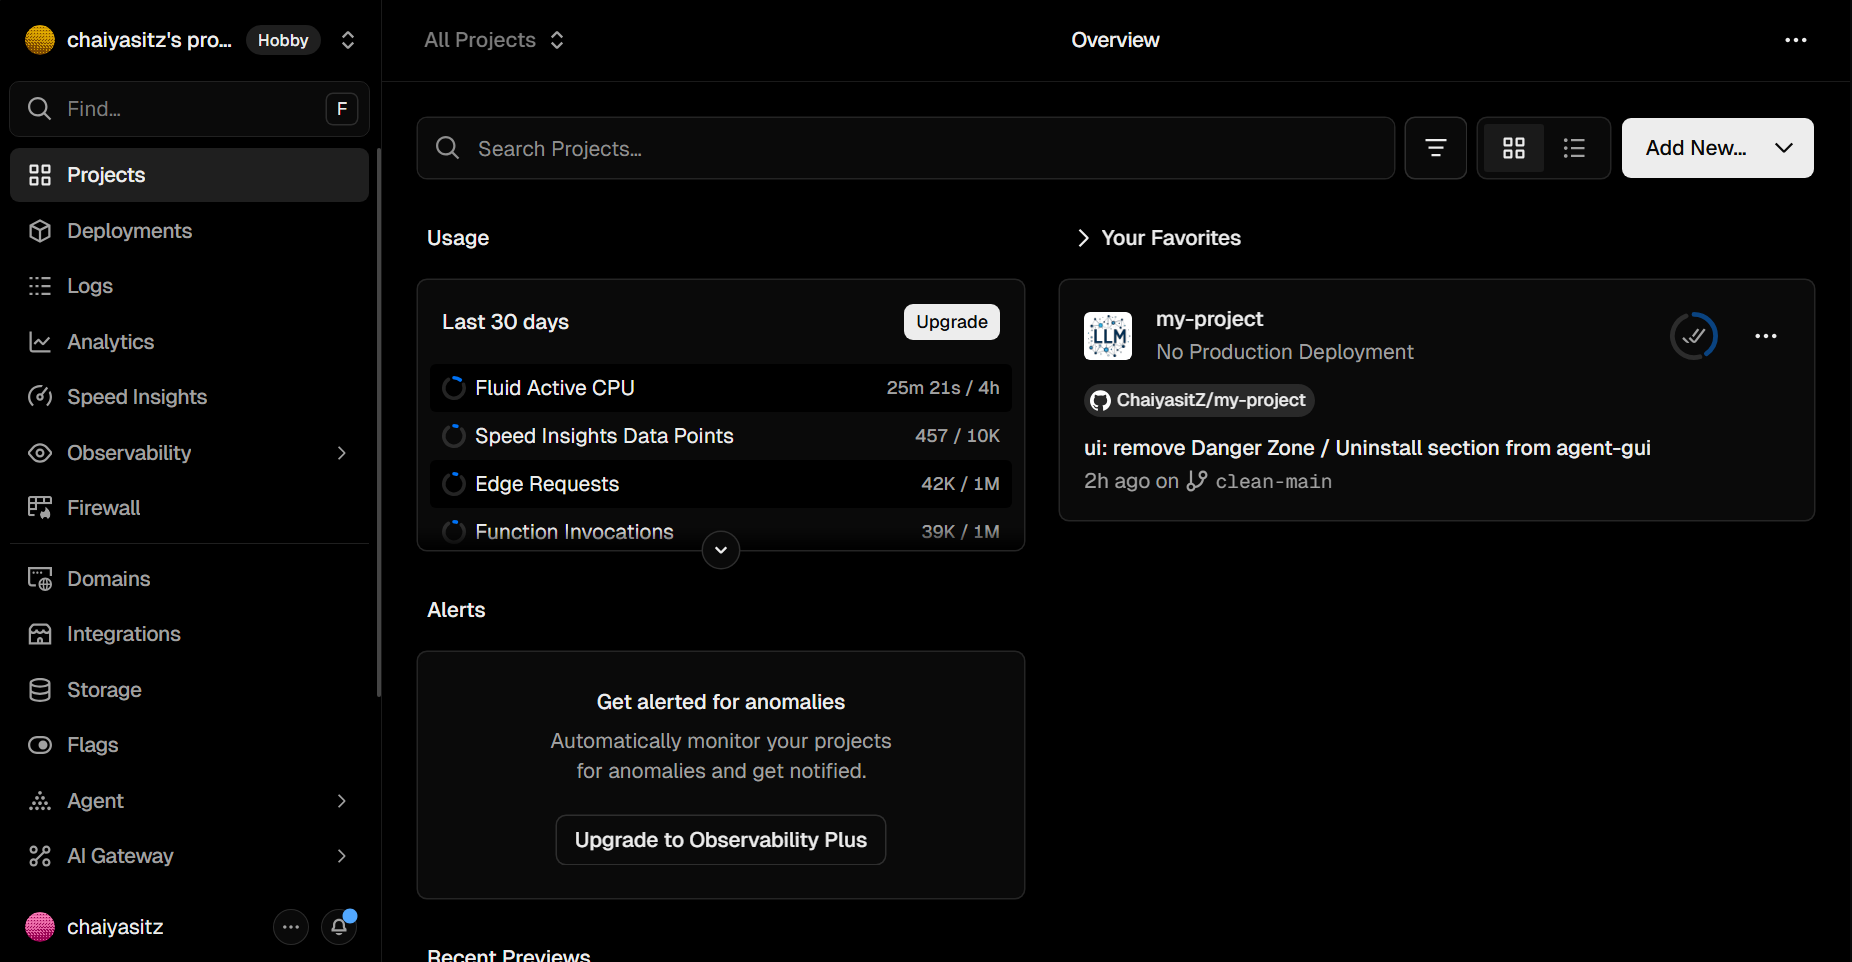
\includegraphics[width=1.0\textwidth]{Image/vercel-3.png}
}
\caption{\fontSixTeen{หลังจากกด Import รอสักพักจน Import เสร็จตัวโปรเจคจะเข้าไมอยู่ใน Vercel}}
\label{figB:Vercel7}
\end{figure}

\begin{figure}[H]
\centering
\adjustbox{frame, width=1.0\textwidth}{
    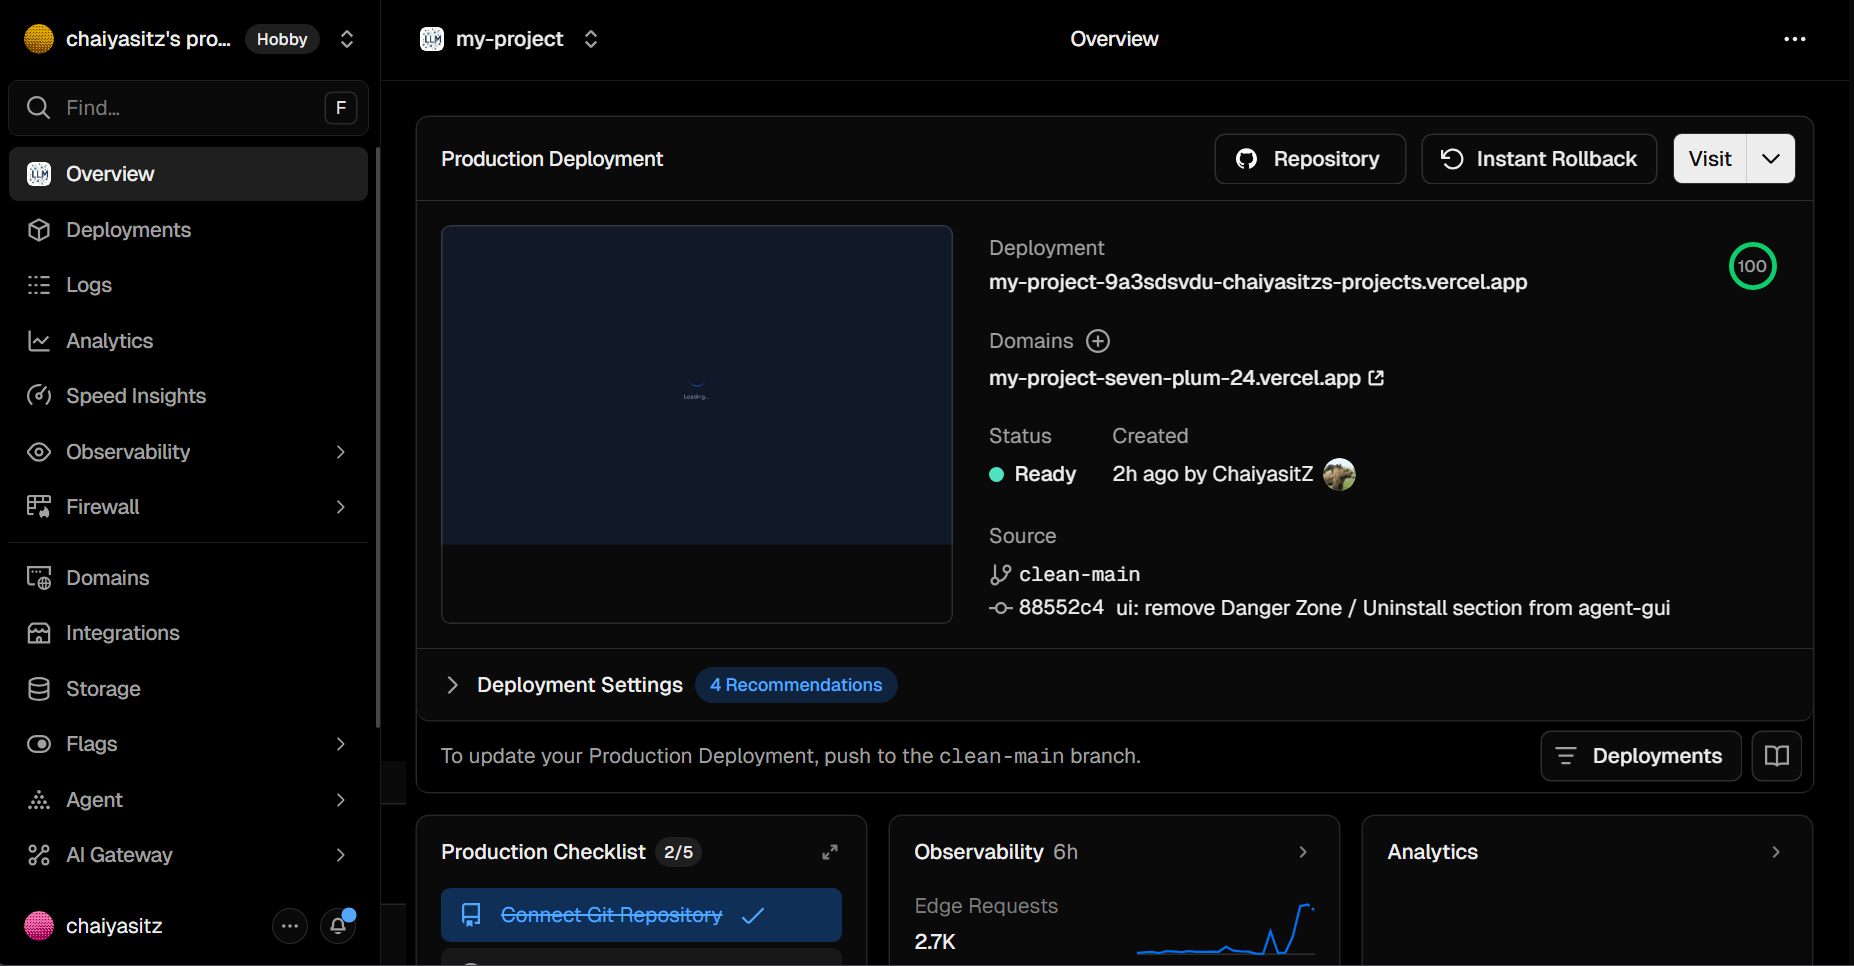
\includegraphics[width=1.0\textwidth]{Image/vercel-4.png}
}
\caption{\fontSixTeen{จะได้ตัวโปรเจคพร้อมโดเมนฟรีสำหรับเข้าใช้งานตัวโปรเจค}}
\label{figB:Vercel8}
\end{figure}